\documentclass{FEIbeamer}

\title{Introdução à Maratona de Programação}
\subtitle{Maratona de Programação FEI}
\author[cferreira@fei.edu.br]{Prof. Charles Ferreira}
\usepackage{hyperref}
\hypersetup{
    colorlinks = true,
    linkcolor = black,
    urlcolor  = blue,
    citecolor = blue,
anchorcolor = blue}
\begin{document}

\section{Maratona de Programação}

\begin{frame}[fragile]{Objetivo}

    \textbf{Treinar equipes para competir em maratonas de programação}
    \bi%
    @ Treinar resolução de problemas
    @ Aprender sobre computação
    \ei%
\end{frame}

\begin{frame}[fragile]{No último fim de semana ...}

    \textbf{Participamos da Regional de São Paulo (71 times competindo)}

    \vspace{-0.5cm}
    \centralize{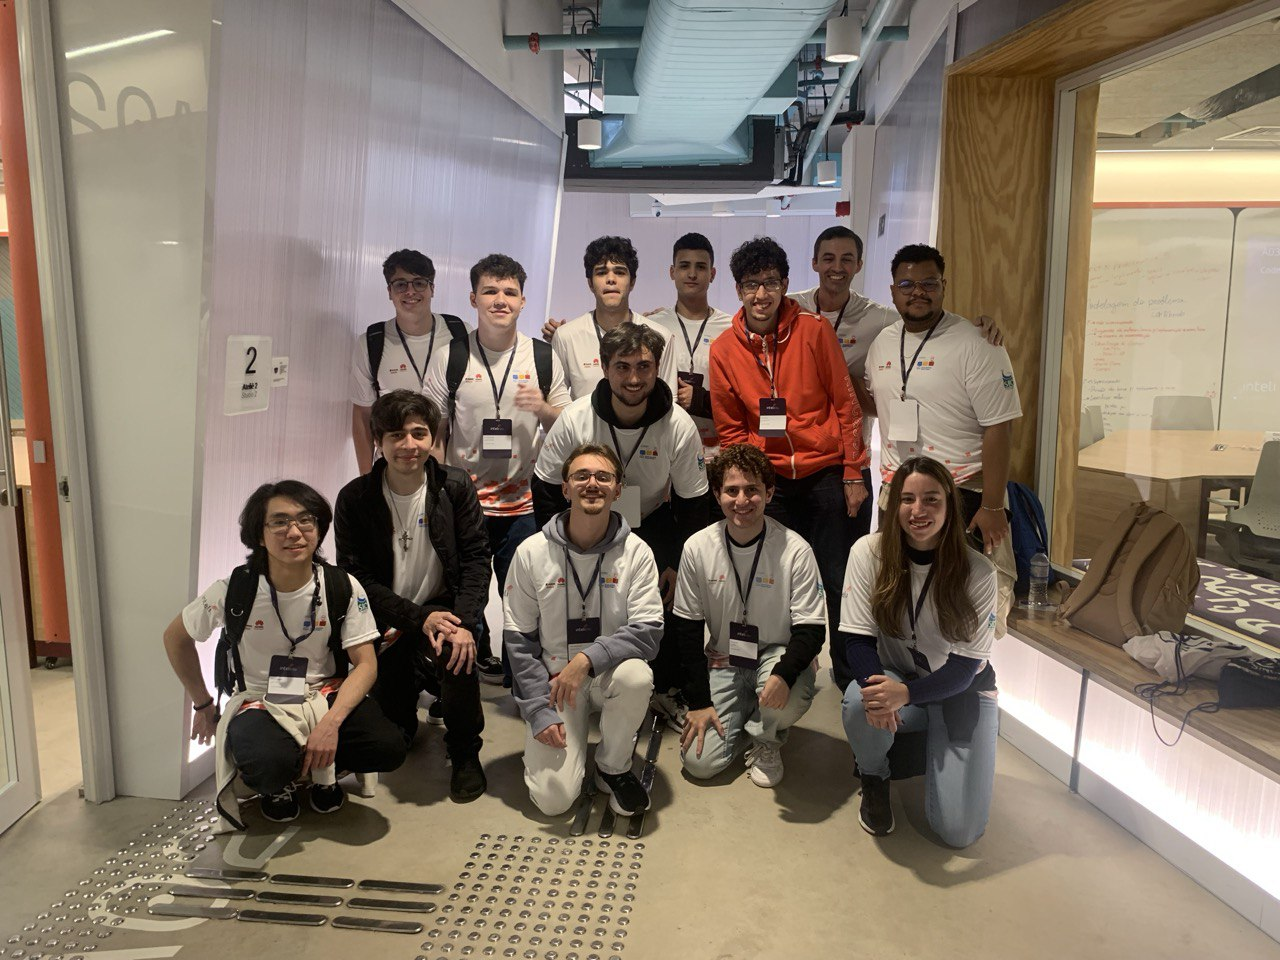
\includegraphics[scale=0.20]{imagens/regional.jpg}}

    \pause

    \floatnode[]{\feibox{Conquistamos uma vaga\\ na final nacional!!!}}

\end{frame}


\section{Problemas da Maratona de Programação}

\begin{frame}[fragile]{Sites de competição}
    \textbf{Materiais de estudo e exercícios para aperfeiçoamento}\pause
    \bi%
    @ \url{beecrowd.com} (Beecrowd)
    \raisebox{-10pt}{
\includegraphics[scale=0.25]{imagens/beecrowd.png}}\pause
    @ \url{https://usaco.guide/} (USACO)
    \raisebox{-5pt}{
\includegraphics[scale=0.3]{imagens/usaco.png}}\pause
    @ \url{https://cses.fi/} (CSES)
    \raisebox{-3pt}{
\includegraphics[scale=0.3]{imagens/cses.png}}\pause
    @ \url{https://youkn0wwho.academy/topic-list} (YouKnowWho Academy)
    \raisebox{-3pt}{
\includegraphics[scale=0.3]{imagens/youknowhwo.png}}\pause
    @ \url{https://codeforces.com/} (CodeForces)
    \raisebox{-3pt}{
\includegraphics[scale=0.3]{imagens/codeforces.png}}
    \ei%
\end{frame}

\begin{frame}[fragile]{Material de Apoio}

    \textbf{Página do github (em construção - maratona-programacao-fei)}
    \bi%
    @ Material de apoio 
    @ Informações compartilhadas
    \ei%
    \floatnode[x=10,y=4]{
\includegraphics[scale=1.0]{imagens/githug.pdf}}
\end{frame}

\begin{frame}[fragile]{}
    \question{E como é um problema da maratona de programação}
\end{frame}

\begin{frame}[fragile]{Exemplo: Problemas de competição}
    \textbf{Basicamente um problema da maratona é constituído de três partes}
    \bi%
    @ Enunciado (descrição do problema)
    @ Conjunto de Entradas
    @ Saída esperada
    \ei%
\end{frame}

\begin{frame}[fragile]{Enunciado: Exemplo}
    \centralize{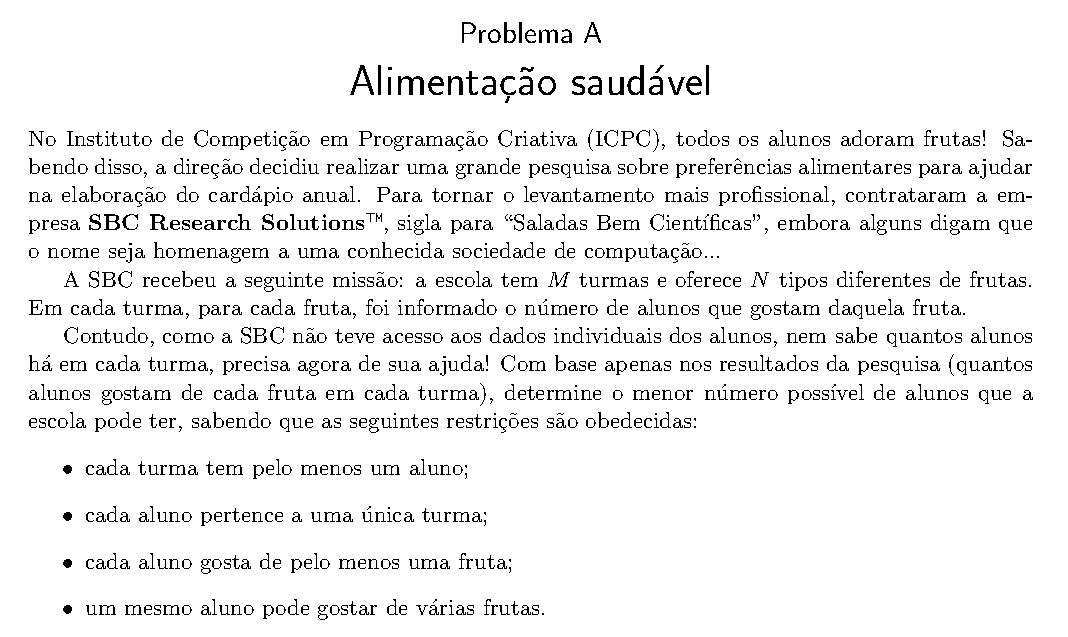
\includegraphics[scale=0.70]{imagens/exemplo_maratona_problema_A.pdf}}
    % \grid
    \balloon[xshift=-1.15,x=6.5,y=12.5]{Alguns problemas\\ costumam \\ser longos}
    % \balloon[xshift=2,x=12.5]{Importante saber\\ler em inglês}
\end{frame}

\begin{frame}[fragile]{Entrada: Exemplo}
    \centralize{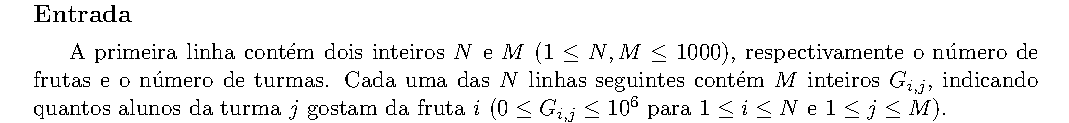
\includegraphics[scale=0.85]{imagens/exemplo_maratona_A_entrada.pdf}}
\end{frame}

\begin{frame}[fragile]{Saída: Exemplo}
    \centralize{
        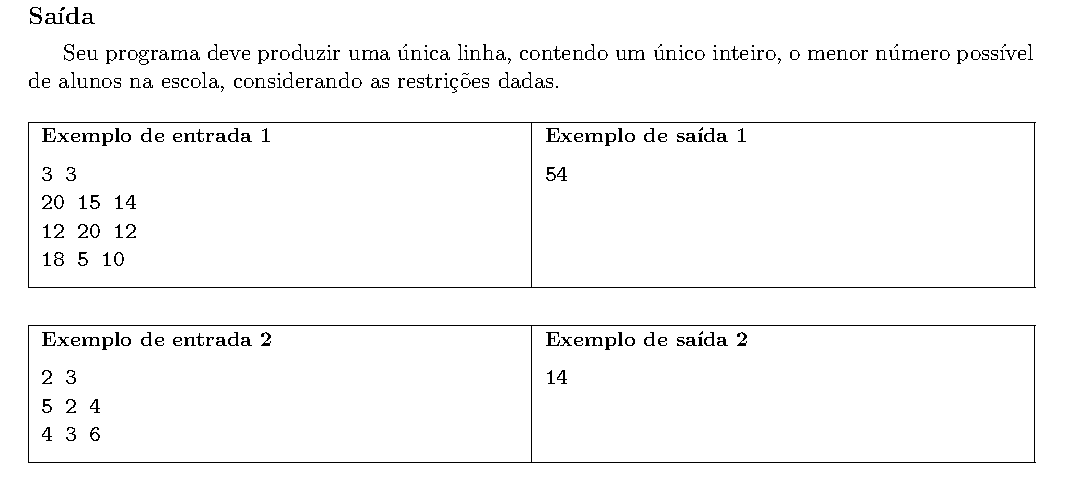
\includegraphics[scale=0.8]{imagens/exemplo_maratona_A_saida.pdf}

        % 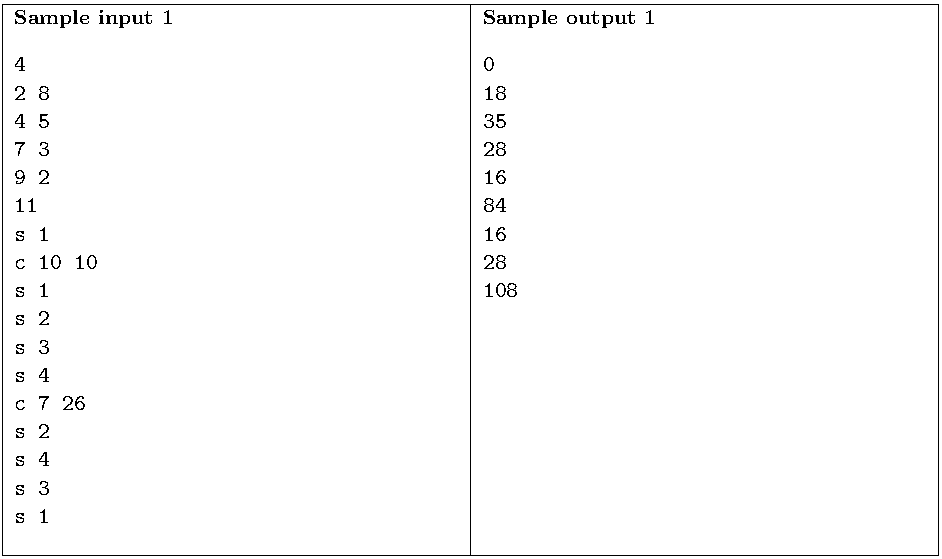
\includegraphics[scale=0.6]{imagens/exemplo_maratona-output2.pdf}
    }
\end{frame}


\section{Linguagens de Programação}

\begin{frame}[fragile]{Linguagens}
    \textbf{Geralmente as linguagens mais comuns são:}
    \Activate\doublecolumn[0.5]{%
        \bi%
        @ \tikzmarknode[anchor=east]{escolha}{C++}
        @ C
        @ Java
        \ei
    }{% ---------
        \bi
        @ Python
        @ Kotlin
        @ \tikzmarknode[anchor=south east]{outras}{Outras}
        \ei%
    }\Deactivate
    \pause
    \balloon[follow=escolha,xshift=3,yshift=0]{Nossa escolha:\\devido ao desempenho\\e as bibliotecas (STL)}
    \pause
    \balloon[x=8,y=2,xshift=1.5,yshift=-1.5,follow=outras]{Interessante ter conhecimentos sobre\\ alguma outra linguagem além de C++}
\end{frame}

\begin{frame}[fragile]{Compilação e execução de programas}
    \textbf{Habilidades que serão desenvolvidas e aperfeiçoadas}\pause
    \bi%
    @ Linux (Sistema Operacional usado na competição)\pause
    @ Utilizar o terminal
    \floatnode[x=14.5,y=5.5]{
\includegraphics[scale=0.3]{imagens/terminal.png}}
    \\\hrulefill \pause
    @ Compilar um programa pela linha de comando\pause
    @ Executar um programa pela linha de comando\pause
    @ Entender os erros do compilador
    % @ Fazer scripts em bash
    \ei%
\end{frame}


\section{Editores de Texto}

% comentar sobre editores de modo geral
% mostrar o vim
% comentar brevemente sobre suas vantagens

\begin{frame}[fragile]{Editores de texto}
    \textbf{Princípio importante:}

    \feibox{Qualquer editor de texto lhe serve}

    É importante que o editor de texto seja um acelerador e não uma muleta!
\end{frame}

\begin{frame}[fragile]{Editores usados comumente}
    \textbf{Nosso laboratório possui:} 
    \Activate\doublecolumn[0.5]{%
        \bi%
        @ \tikzmarknode[anchor=south east]{vim}{VIM} 
        @ NeoVim
        \ei
    }{% ---------
        \bi
        @ Gedit
        @ VS Code
        % @ Code Blocks
        \ei
    }\Deactivate
    % \balloon[follow=vim,yshift=-2,xshift=4]{Costumamos usar\\com mais frequência}
\end{frame}

\begin{frame}[fragile]{Vi IMproved}
    \floatnode[x=10,y=7]{
\includegraphics[scale=0.3]{imagens/vim.png}}
    \textbf{Principais características} \pause
    \Activate\doublecolumn[0.4]{%
        \bi%
        @ Roda no terminal \cmark\pause
        @ Keyboard Driven \cmark\pause
        @ Modular \cmark\pause
        @ Programável \cmark\pause
        \ei%
    }{% --------- 
        \bi%
        @ Tem uma curva de aprendizado grande \xmark\pause
        @ Não é amigável (inicialmente) \xmark
        \ei%
    }\Deactivate
\end{frame}

\section{Digitação}

% comentar sobre a importância de saber digitar sem olhar
% fazer alguns exercícios básicos de digitação 
% recomendar o site do typing club

\begin{frame}[fragile]{Aprender a digitar}
    \textbf{Importante fazer um curso de digitação}
    \bi%
    @ Aprender a digitar com as duas mãos
    @ Posicionar as mãos corretamente
    @ Recomendação: \url{typingclub.com} (existem outros)
    \ei%
\end{frame}

\begin{frame}[fragile]{Exercício de digitação}
    \textbf{Vamos fazer um pequeno experimento \ldots}
    \bi%
    @ Abra um editor de texto qualquer (gedit, notepad, etc.)
    @ Posicione suas mãos no teclado como faria normalmente para digitar
    \ei%
    \centralize{
\includegraphics[scale=0.15]{imagens/typing-icon.png}}
\end{frame}

\begin{frame}[fragile]{Exercício de digitação}
    \textbf{Tente digitar o seguinte texto sem olhar para o teclado}\pause

    \lstset{language=c}
    \code[space=0.5,size=1.2]{codes/treino_digitacao.cpp}

\end{frame}

\section{Rotina de estudos}

% comentar da importância da rotina de estudos
% apresentar a planilha do bernardo como sugestão de estudos
% mostrar os horários da maratona

\begin{frame}[fragile]{Rotina de estudos}
    \textbf{Importante criar uma rotina de estudos}
    \bi%
    @ Equilíbrio entre resolver exercícios e aprender novos conceitos
    \ei%
    \feibox{Consistência vence intensidade!}
    \bi%
    @ Melhor treinar pouco frequentemente do que muito em um único dia.
    \ei%
\end{frame}

\begin{frame}[fragile]{Sugestão de treinamento inicial}
    \textbf{Planilha de controle de estudos}
    \bi%
    @ Link: \href{https://docs.google.com/spreadsheets/d/1vIG3zgXMlWQHlMUfeSqw3-CEygCgLByi0B3yTgbtMZo/edit?usp=sharing}{Google Sheets}
    @ Solicite a adição de uma aba com o seu nome
    @ Va marcando os exercícios que já conseguiu resolver \cmark
    \ei%
    \floatnode[x=13,y=6]{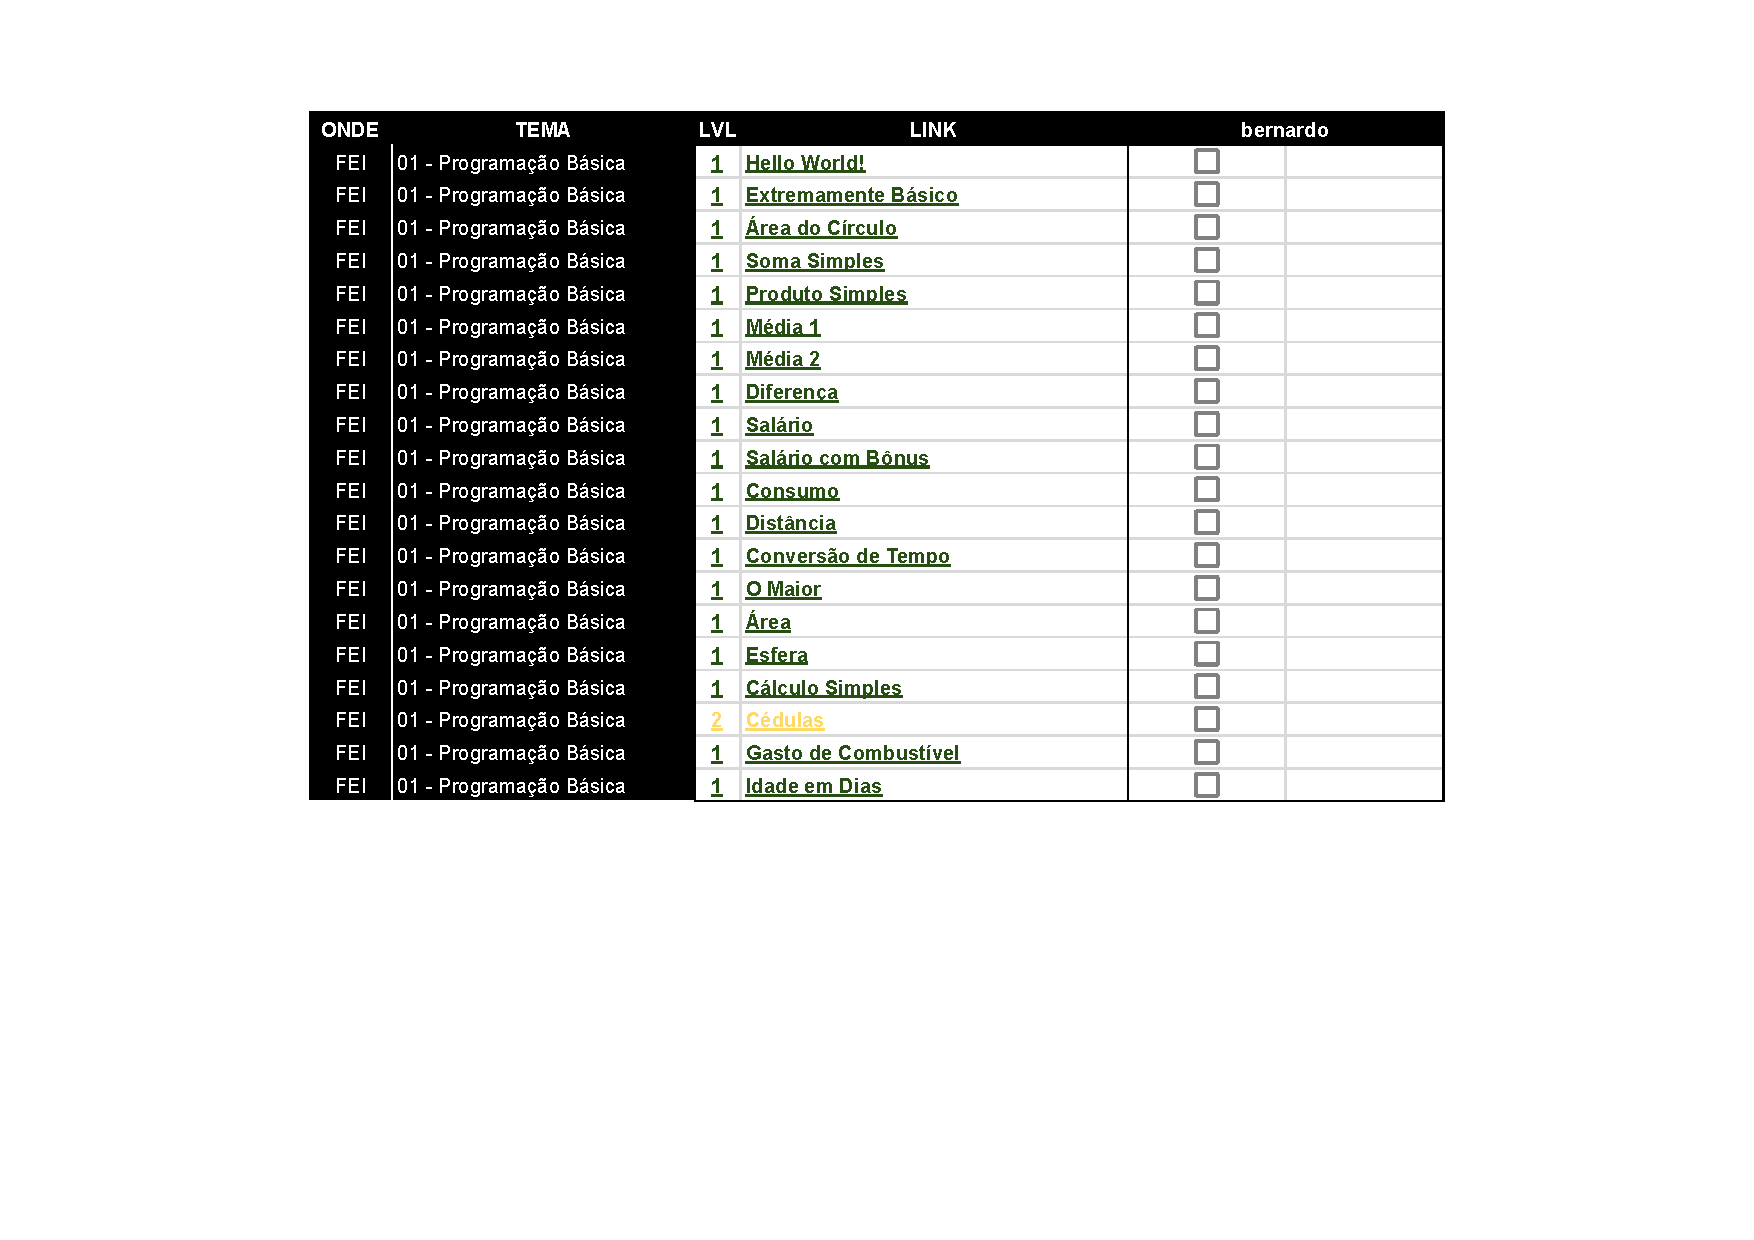
\includegraphics[scale=0.25]{imagens/ProgressoMaratona-Beecrowd.pdf}}
\end{frame}

\begin{frame}[fragile]{Sugestão de treinamento inicial}
    \floatnode[x=13,y=4]{
\includegraphics[scale=0.10]{imagens/productivity-expert-icon.png}}
    \textbf{Ao travar por muito tempo em algum problema:} \pause
    \bi%
    @ Tente conversar com quem já resolveu.\pause
    @ Procure entender a descrição da solução.\pause
    @ Rabisque em um papel ou na lousa.\pause
    @ Por fim, tente efetivamente codificar.
    \ei%
\end{frame}

\section{Encontros (contéudo programático)}

\begin{frame}[fragile]{Encontros}
    \textbf{Sala da Maratona: K409}
    \bi%
    @ Horário de treinamento:

    \vspace{-0.5cm}\hrulefill
    @@ Segunda - Sexta: 13:00 às 18:00
    @@ Responsáveis: Gabriel e %\inlinepic{example-image-a}{0.1}
    Alexandre %\inlinepic{example-image-a}{0.1} e 

    \vspace{-0.5cm}\hrulefill
    @@ Segunda - Sexta: 09:30 às 12:00
    @@ Responsáveis:  %\inlinepic{example-image-a}{0.1} e 
    Bernardo e %\inlinepic{example-image-a}{0.1}
    Rafael% \inlinepic{example-image-a}{0.1}
    \ei%
    \floatnode[x=12,y=7]{
\includegraphics[scale=0.1]{imagens/keys-icon.png}}
\end{frame}

% \begin{frame}[fragile]{Cronograma}
%     \centralize{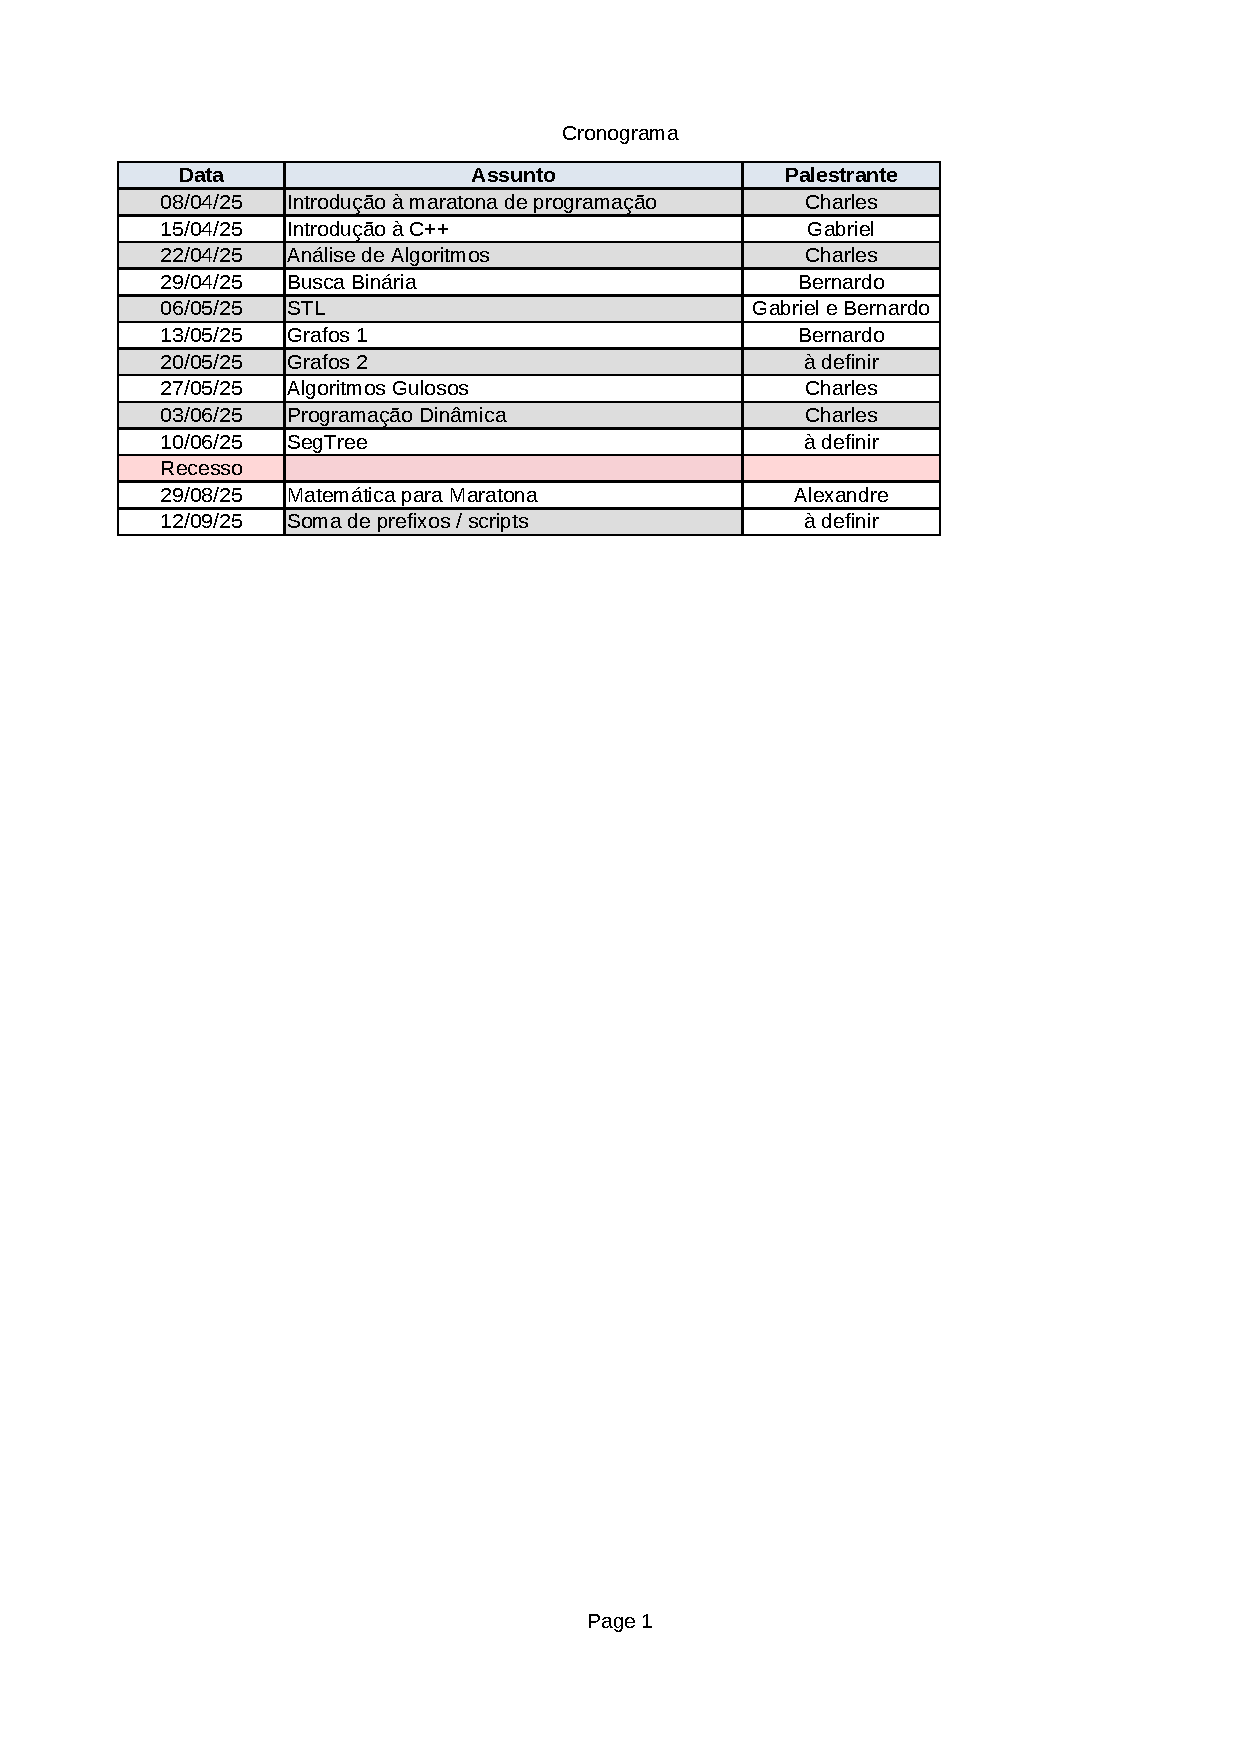
\includegraphics[scale=0.8]{imagens/cronograma_aulas.pdf}}
% \end{frame}

\end{document}
